\section{衡量词向量的语法和语义规律}
\label{sec:mea-syn-and-sem-reg}
相比于经典$n$-gram模型所使用的独热编码, 词向量的一个主要优势就是依靠连续空间表示实现了泛化
\cite{Bengio2006}。
这种泛化体现在,相似的词不仅彼此的距离很近,而且还有多维度的相似性
\cite{DBLP:conf/naacl/MikolovYZ13}。
换句话说,一个词向量可以编码多种类型的关系,如 \cref{fig:word-offsets} 所示。
具体来说,词向量既可以编码语法规律(syntax regularity),例如单复数关系和词性关系,
也可以编码语义规律(semantic regularity),例如首都和国家关系以及性别关系。

目前,计算并衡量这些关系的主流方法是一个简单的向量偏移方法
\cite{DBLP:conf/naacl/MikolovYZ13}。假设词$x_a$和$x_b$具有某种关系,而词$x_c$和$x_d$
具有相同的关系,那么 $x_a - x_b + x_c$将得到一个离$x_d$最近的词向量。
例如,对于具有性别关系的两个词对$(King, Queen)$和$(Man, Woman)$来说,
$vector("King") - vector("Man") + vector("Woman")$将得到一个离Queen最近的词向量。

为了衡量词向量的语法和语义规律,Mikolov等人提出了一种基于类比问题的测试集。这种类比问题
给出了一对具有某个关系的词,要求得出具有相同关系的,和另一个词最接近的词,比如回答
“给定Man-Woman关系,在此关系上和King最接近的词是?”。
在 \cite{DBLP:conf/naacl/MikolovYZ13}中
Mikolov等人设计了一个语法测试集,并取得了接近40\%
\footnote{Mikolov等人把完全匹配视为正确回答,并不使用近义词。}
的准确率。

具体来说,为了回答类比问题$a:b\  c:d$($d$是未知的),该方法
寻找词向量$x_a,x_b,x_c$(都已正则化为单位模长),并计算 $y=x_b-x_a+x_c$,
然后查找和$y$的cosine相似度最大的向量并输出对应的词:
\begin{align*}
  w^{*} = argmax_w \frac{x_w y}{\lVert x_w \rVert \lVert y \rVert}
\end{align*}
当词向量训练的足够好时,这种方法可以找到正确答案。

总的来说,这种向量偏移方法具有以下优点:
\begin{enumerate}
  \item 扩展了分布式假设中对含义的理解,用词相似性的类比(analogy of word similarity)
    衡量词向量捕获的语言规律,很好的解释了词向量的含义问题。
  \item 把语言实体之间多种复杂的关系简化为实向量空间的线性关系,实现了
    利用表征学习降维的目的\cite{HinSal06}。
  \item 向量操作简单,直观,容易实现。
\end{enumerate}

\begin{figure}
  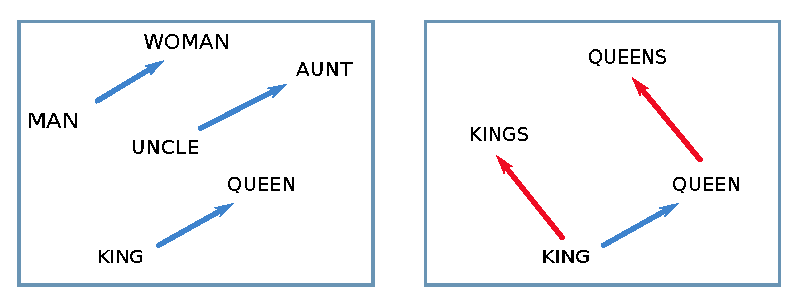
\includegraphics[width=0.8\textwidth]{figures/word-offsets.eps}
  \centering
  \caption{词向量在向量空间的直观示意图。同一个词向量可以编码多种关系
  \cite{DBLP:conf/naacl/MikolovYZ13}}
  \label{fig:word-offsets}
\end{figure}

